% Manual of pgf-pie.sty, a convenient set of macros for drawing pie
% chart. Written by Xu Yuan <xuyuan.cn@gmail.com> This file is part of
% pgf-pie you may get it at http://code.google.com/p/pgf-pie/

\documentclass{article}
\usepackage[margin=12mm]{geometry}
\usepackage{hyperref}

\usepackage{pgf-pie}
\usetikzlibrary{shadows}

%%%%%%%%%%%%%%%%%%%%%%%%%%%%%%%%%%%%%%%%%%%%%%%%%%%%%%%%%%%%%%%%%
\usepackage{listings}
\usepackage{color}
\definecolor{listinggray}{gray}{0.92}
\lstset{ %
language=[LaTeX]TeX,
breaklines=true,
frame=single,
% frameround=tttt,
basicstyle=\footnotesize\ttfamily,
backgroundcolor=\color{listinggray},
keywordstyle=\color{blue}
}
%%%%%%%%%%%%%%%%%%%%%%%%%%%%%%%%%%%%%%%%%%%%%%%%%%%%%%%%%%%%%%%%%

%%%%%%%%%%%%%%%%%%%%%%%%%%%%%%%%%%%%%%%%%%%%%%%%%%%%%%%%%%%%%%%%%
\hypersetup{
  colorlinks=true,
  linkcolor=blue,
  anchorcolor=black,
  citecolor=olive,
  filecolor=magenta,
  menucolor=red,
  urlcolor=blue
}
%%%%%%%%%%%%%%%%%%%%%%%%%%%%%%%%%%%%%%%%%%%%%%%%%%%%%%%%%%%%%%%%%

%%%%%%%%%%%%%%%%%%%%%%%%%%%%%%%%%%%%%%%%%%%%%%%%%%%%%%%%%%%%%%%%%
\newcommand{\demo}[2][1]{
  \begin{center}
  \begin{tabular}{cc}
    \begin{minipage}{.49\linewidth}
      \centering
      \resizebox{#1\linewidth}{!}{
        \input{demo/#2}
      }
    \end{minipage}
    &
    \begin{minipage}{.45\linewidth}
      \lstinputlisting{demo/#2}
    \end{minipage}
  \end{tabular}
  \end{center}
}
%%%%%%%%%%%%%%%%%%%%%%%%%%%%%%%%%%%%%%%%%%%%%%%%%%%%%%%%%%%%%%%%%

%%%%%%%%%%%%%%%%%%%%%%%%%%%%%%%%%%%%%%%%%%%%%%%%%%%%%%%%%%%%%%%%%
\newcommand{\example}[2][1]{
  \begin{center}  
    \resizebox{#1\linewidth}{!}{
      \input{demo/#2}
    }
  \end{center}
  \lstinputlisting{demo/#2}
}
%%%%%%%%%%%%%%%%%%%%%%%%%%%%%%%%%%%%%%%%%%%%%%%%%%%%%%%%%%%%%%%%% 

\begin{document}
%%%%%%%%%%%%%%%%%%%%%%%%%%%%%%%%%%%%%%%%%%%%%%%%%%%%%%%%%%%%%%%%%
\title{Drawing Pie Chart by using \texttt{pgf-pie}}
\author{\href{mailto:xuyuan.cn@gmail.com}{Yuan Xu}}
\date{\today{}~(v0.1)}
\maketitle
%%%%%%%%%%%%%%%%%%%%%%%%%%%%%%%%%%%%%%%%%%%%%%%%%%%%%%%%%%%%%%%%%

\begin{abstract}
  \texttt{pgf-pie} is a LaTeX package for drawing pie chart. As stated
  by its name, it is based on a very popular graphic package
  \texttt{PGF/TikZ}. This document presents the usage of
  \texttt{pgf-pie} and collects some pie charts as examples.
  \texttt{pgf-pie} can be downloaded from
  \href{http://code.google.com/p/pgf-pie/}{http://code.google.com/p/pgf-pie/}.
\end{abstract}

\tableofcontents

\section{The Essentials}

\subsection{First Pie}
\demo[0.6]{first-pie}

\subsection{Position, Rotation, Size}

The center of chart can be set by \texttt{pos}, default is
\texttt{\{0,0\}}. The chart can be rotated by setting \texttt{rotate}
(in degrees). The size of chart can be set by \texttt{radius}, default
is 3.

\demo{radius}

\subsection{Explode}
\demo{explode}

\subsection{Text Label}

\subsubsection{Text inside pie}
\demo[0.6]{before-after-number}

\subsubsection{Text outside pie}
The value of \texttt{text} can be \texttt{label}(default) or
\texttt{pin}.

\demo[0.6]{text}

\subsection{Sum}
The value of \texttt{sum} indicats the sum of all data in the chart,
it is 100 by default. It can be calculated automatically when
\texttt{auto} is set.

\demo{sum}

\subsection{Color}
The color can be specified by \texttt{color}, the default color wheel
is shown in figure \ref{fig:color-wheel}.

\demo{color}


\begin{figure}
  \centering
  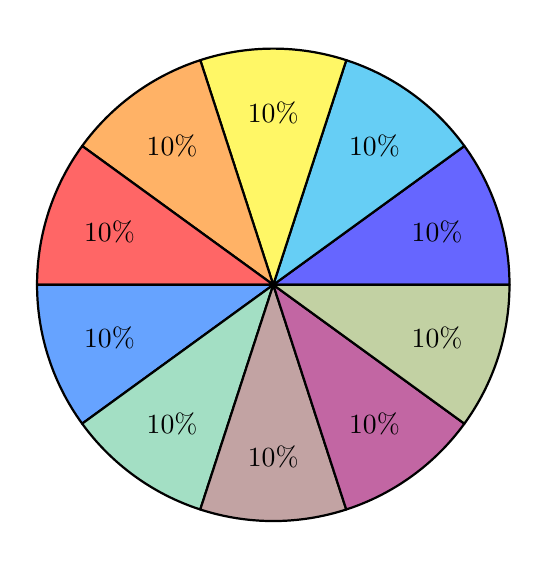
\begin{tikzpicture}
  \pie{10/, 10/, 10/, 10/, 10/, 10/, 10/, 10/, 10/, 10/}
\end{tikzpicture}
  \caption{Default color wheel}
  \label{fig:color-wheel}
\end{figure}


\subsection{Style}
\subsubsection{shadow}
\demo[0.6]{shadow}

\section{Examples}

% \subsection{Population of the world}
% \example{population}

% \section{Acknowledgements}
% Many people contributed to \texttt{pgf-pie} by reporting problems,
% suggesting various improvements or submitting code. Here is a list of
% these people:
% \href{mailto:???}{name}.

\end{document}
%%% Local Variables: 
%%% mode: Tex-PDF
%%% TeX-master: t
%%% End: 
